\chapter{Catálise homogênea na indústria}\label{ch:b3:homogeneous-catalysis}

A maior parte do ácido acético do mundo, matéria-prima do acetato de vinila, do
acetato de celulose e do ácido tereftálico purificado das garrafas plásticas, é
produzida a partir de metanol e monóxido de carbono em algumas poucas fábricas muito grandes. Em cada uma, um
complexo de ródio ou de irídio dissolvido em baixa concentração no líquido
reacional realiza milhares de ciclos por hora, durante anos. O mesmo tipo de
química hidrogena, adiciona CO e hidrogênio a alquenos, troca as extremidades de
ligações duplas, une anéis aromáticos e produz polietileno e polipropileno aos
milhões de toneladas. Este capítulo lê os ciclos catalíticos dos principais
processos industriais com as ferramentas do \cref{ch:b3:organometallic-bonding}:
contagens de elétrons, estados de oxidação, etapas determinantes da velocidade e a simetria do
catalisador que fixa a estrutura de um polímero.

\begin{recall}
O volume do 2.º ano introduziu as etapas elementares das reações organometálicas
(adição oxidativa, eliminação redutiva, inserção migratória, eliminação de
$\beta$-hidreto, transmetalação), os ciclos catalíticos, os pré-catalisadores, o número
e a frequência de rotação, e leu os ciclos da hidrogenação, da \omterm{def:b3:homogeneous-catalysis:hydroformylation}{hidroformilação} e do
acoplamento cruzado; definiu também a taticidade e a polimerização em cadeia,
a conversão e a seletividade. O \cref{ch:b3:organometallic-bonding} contou os
elétrons e descreveu os ligantes carbonila e \omterm{def:b3:organometallic-bonding:carbene}{carbeno};
o \cref{ch:b3:complex-kinetics} deu a cinética de saturação;
o \cref{ch:b3:point-groups}, os \omterm{def:b3:point-groups:operation}{elementos de simetria} das moléculas.
\end{recall}

\begin{omfigure}
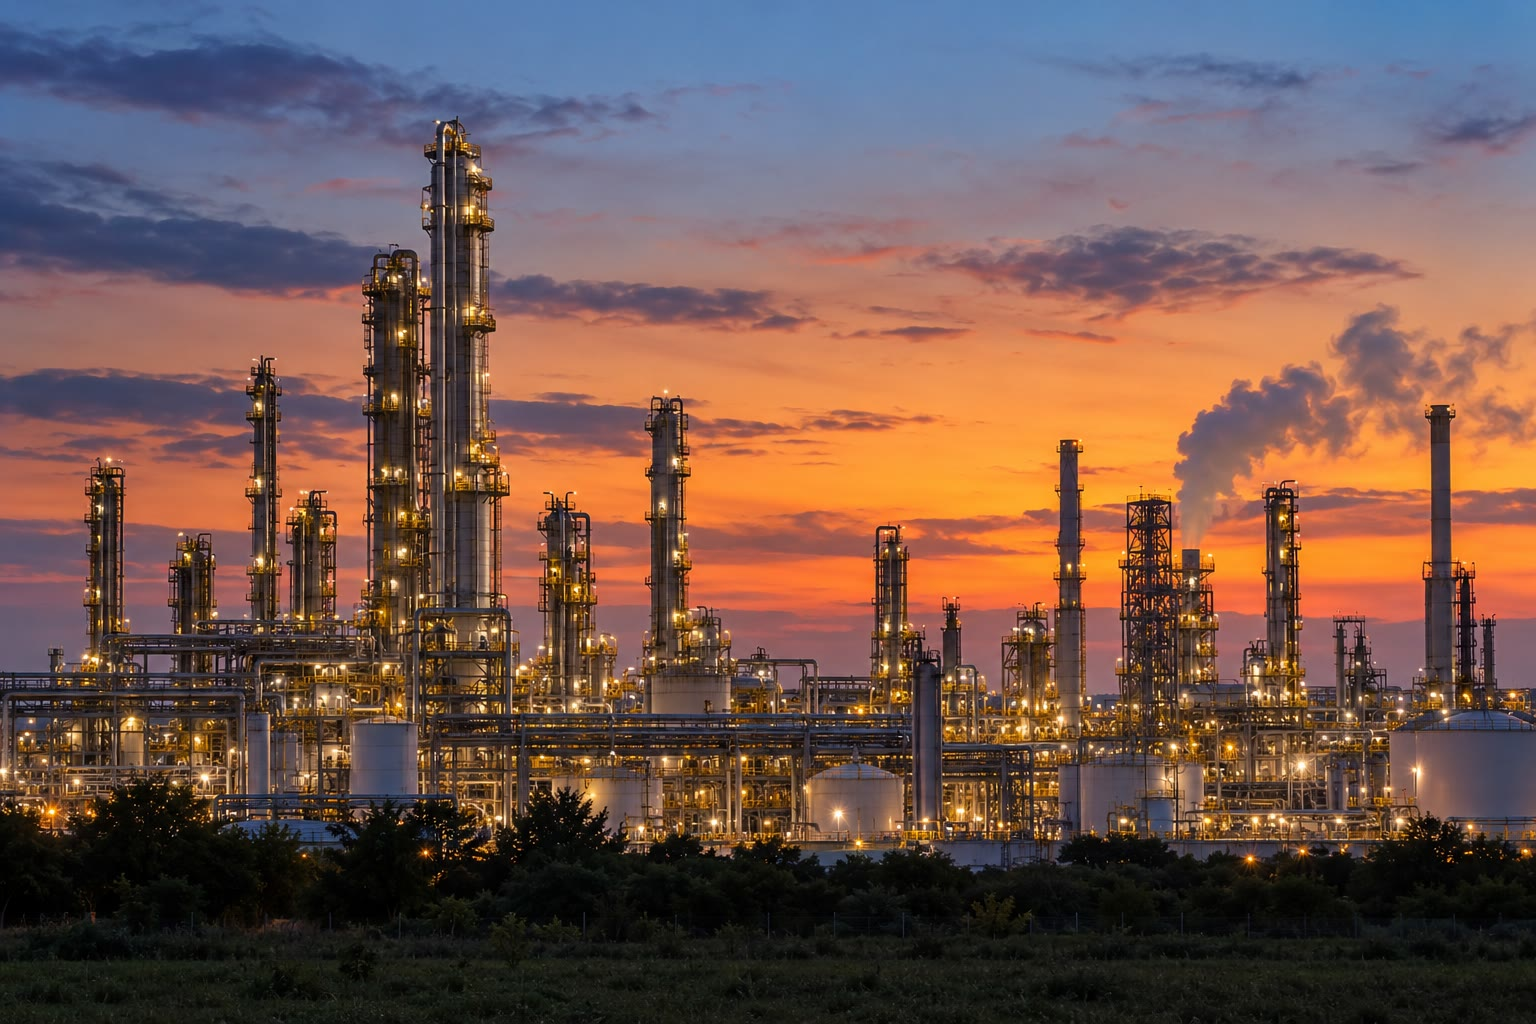
\includegraphics[width=0.6\linewidth]{images/book4/ai/b3-21-chemical-plant.jpg}

{\small Uma grande fábrica química ao entardecer. Em uma unidade de \omterm{def:b3:homogeneous-catalysis:carbonylation}{carbonilação}, o catalisador
é um complexo metálico dissolvido no líquido reacional; a maior parte da fábrica
separa e recicla.}
\end{omfigure}

\section{Hidrogenação}

\begin{method}[Ler um ciclo catalítico]\label{met:b3:homogeneous-catalysis:read-cycle}
\begin{enumerate}
  \item Em cada espécie, conte os elétrons de valência e dê o estado de oxidação
        e o $d^n$ do metal.
  \item Nomeie cada etapa (perda ou adição de ligante, adição oxidativa,
        inserção, eliminação) e verifique que as contagens mudam como ela exige
        (adição oxidativa: $+2$ no estado de oxidação e na contagem de elétrons).
  \item Identifique o estado de repouso (a espécie que se acumula) e a
        etapa determinante da velocidade; a lei de velocidade decorre dos pré-equilíbrios
        entre eles.
\end{enumerate}
\end{method}

\begin{omfigure}
\begin{tikzpicture}[font=\small, >=Stealth]
  \node (a) at (90:2.3) {\ce{RhCl(PPh3)2} \ (14, Rh$^{\mathrm I}$)};
  \node (b) at (0:3.0) {\ce{RhClH2(PPh3)2} \ (16, Rh$^{\mathrm{III}}$)};
  \node (c) at (-90:2.3) {\ce{RhClH2(RCH=CH2)(PPh3)2} \ (18)};
  \node (d) at (180:3.1) {\ce{RhClH(CH2CH2R)(PPh3)2} \ (16)};
  \draw[->, thick] (a) to[bend left=22] node[midway, above right, font=\scriptsize] {$+\,\ce{H2}$, adição oxidativa} (b);
  \draw[->, thick] (b) to[bend left=22] node[midway, below right, font=\scriptsize] {$+$ alqueno} (c);
  \draw[->, thick] (c) to[bend left=22] node[midway, below left, font=\scriptsize] {inserção migratória} (d);
  \draw[->, thick] (d) to[bend left=22] node[midway, above left, font=\scriptsize, align=right] {eliminação\\ redutiva: $-$ alcano} (a);
  \node[anchor=south] (p) at (90:3.4) {\ce{RhCl(PPh3)3} \ (16, pré-catalisador)};
  \draw[<->, black!50] (p) -- (a) node[midway, right, font=\scriptsize] {$\mp\,\ce{PPh3}$};
\end{tikzpicture}

{\small Um ciclo simplificado da hidrogenação de alquenos pelo catalisador de Wilkinson
(contagens de elétrons de valência entre parênteses). A perda de uma fosfina abre um sítio; o
ciclo adiciona hidrogênio, liga o alqueno, insere-o em uma ligação Rh--H e
elimina o alcano.}
\end{omfigure}

\begin{proposition}[Cinética de Wilkinson]\label{prop:b3:homogeneous-catalysis:wilkinson-rate}
Se $\ce{RhClL3} \rightleftharpoons \ce{RhClL2} + \mathrm L$ ($K_1$) e $\ce{RhClL2} + \ce{H2} \rightleftharpoons \ce{RhClH2L2}$ ($K_2$) são equilíbrios
rápidos e a reação do di-hidreto com o alqueno (constante de velocidade $k$)
é determinante da velocidade,
\[
  v = \frac{kK_1K_2[\mathrm{Rh}]_{\mathrm{tot}}[\ce{H2}][\text{alqueno}]}{[\mathrm L] + K_1 + K_1K_2[\ce{H2}]},
\]
que satura em hidrogênio e é inibida pela fosfina L adicionada.
\end{proposition}

\begin{proof}
$[\ce{RhClL2}] = K_1[\ce{RhClL3}]/[\mathrm L]$ e $[\ce{RhClH2L2}] = K_2[\ce{H2}][\ce{RhClL2}]$. Escrevendo $[\mathrm{Rh}]_{\mathrm{tot}}$ como a
soma das três espécies e isolando o di-hidreto, chega-se a
$[\ce{RhClH2L2}] =
K_1K_2[\ce{H2}][\mathrm{Rh}]_{\mathrm{tot}}/([\mathrm L] + K_1 + K_1K_2[\ce{H2}])$; a velocidade é $k$ vezes isso vezes a
concentração de alqueno.
\end{proof}

O catalisador de Wilkinson hidrogena os alquenos pouco impedidos muito mais depressa que os
substituídos e deixa intactos os grupos carbonila: a seletividade de um
centro metálico congestionado. Difosfinas quirais transformam a mesma química em
hidrogenação assimétrica (\cref{ch:b3:asymmetric-synthesis}).

\section{Processos de carbonilação}

\begin{definition}[Hidroformilação]\label{def:b3:homogeneous-catalysis:hydroformylation}
A \emph{hidroformilação}\index{hidroformilacao@hidroformilação} é a adição de um átomo de hidrogênio
e de um grupo formila (CHO) a uma ligação dupla C=C, a partir de $\ce{H2}$ e CO, que transforma um
alqueno em um aldeído com um carbono a mais. A \emph{razão
linear/ramificado}\index{razao linear/ramificado@razão linear/ramificado} é a razão entre o aldeído
de cadeia linear e o ramificado.
\end{definition}

Os primeiros processos usavam $\ce{HCo(CO)4}$ a cerca de 150 a \qty{180}{\celsius} e pressões muito
altas. O ródio com trifenilfosfina funciona a cerca de \qty{100}{\celsius} e
pressões muito menores, e dá uma \omterm{def:b3:homogeneous-catalysis:hydroformylation}{razão linear/ramificado} maior: as fosfinas volumosas
favorecem a inserção que põe o metal no carbono terminal.
O propeno dá o butanal, hidrogenado a butanol ou convertido em álcoois
para plastificantes.

\begin{definition}[Carbonilação]\label{def:b3:homogeneous-catalysis:carbonylation}
A \emph{carbonilação}\index{carbonilacao@carbonilação} é a introdução de um grupo carbonila
em uma molécula por reação com o monóxido de carbono, catalisada por um complexo metálico
por meio da inserção migratória do CO.
\end{definition}

A \omterm{def:b3:homogeneous-catalysis:carbonylation}{carbonilação} do metanol a ácido acético, $\ce{CH3OH + CO -> CH3COOH}$, funciona com
ródio (o processo Monsanto) ou irídio (o processo Cativa), com iodeto de metila
como cocatalisador: o iodeto de hidrogênio transforma o metanol em iodeto de metila, o metal
insere CO no grupo metila, e o iodeto de acetila formado é hidrolisado,
liberando de novo HI.

\begin{omfigure}
\begin{tikzpicture}[font=\small, >=Stealth]
  \node (a) at (90:2.1) {$\ce{[M(CO)2I2]-}$ (16)};
  \node (b) at (0:2.9) {$\ce{[CH3M(CO)2I3]-}$ (18)};
  \node (c) at (-90:2.1) {$\ce{[CH3COM(CO)I3]-}$ (16)};
  \node (d) at (180:2.9) {$\ce{[CH3COM(CO)2I3]-}$ (18)};
  \draw[->, thick] (a) to[bend left=22] node[midway, above right, font=\scriptsize, align=left] {$+\,\ce{CH3I}$\\ adição oxidativa} (b);
  \draw[->, thick] (b) to[bend left=22] node[midway, below right, font=\scriptsize] {inserção migratória} (c);
  \draw[->, thick] (c) to[bend left=22] node[midway, below left, font=\scriptsize] {$+$ CO} (d);
  \draw[->, thick] (d) to[bend left=22] node[midway, above left, font=\scriptsize, align=right] {eliminação redutiva\\ $-\,\ce{CH3COI}$} (a);
  \node[anchor=north, align=center, font=\scriptsize] at (0,-2.55) {$\ce{CH3COI + H2O -> CH3COOH + HI}$, \quad $\ce{CH3OH + HI -> CH3I + H2O}$};
\end{tikzpicture}

{\small O ciclo de \omterm{def:b3:homogeneous-catalysis:carbonylation}{carbonilação} do metanol para $\mathrm M = \mathrm{Rh}$ (Monsanto); contagens de
elétrons de valência entre parênteses, estado de oxidação do metal I no alto, III nas demais posições.
Com ródio, a adição oxidativa do iodeto de metila é determinante da velocidade. Com
irídio (Cativa), ela é muito mais rápida, a inserção migratória é lenta, e
\omterm{def:b3:surfaces-catalysis:catalyst-design}{promotores} que retiram um iodeto de $\ce{[CH3Ir(CO)2I3]-}$ aceleram a inserção.}
\end{omfigure}

\begin{proposition}[Lei de velocidade do processo com ródio]\label{prop:b3:homogeneous-catalysis:monsanto-rate}
Se a adição oxidativa do iodeto de metila a $\ce{[Rh(CO)2I2]-}$ é determinante da velocidade e
esse complexo é o estado de repouso, $v = k[\mathrm{Rh}]_{\mathrm{tot}}[\ce{CH3I}]$: ordem zero em CO e em
metanol.
\end{proposition}

\begin{proof}
A velocidade é a da etapa lenta, $k[\ce{[Rh(CO)2I2]-}][\ce{CH3I}]$, e quase todo o ródio
está no estado de repouso. O CO só entra depois da etapa lenta, e o metanol apenas
regenera o iodeto de metila, cuja concentração estacionária é fixada pelo iodeto
carregado no reator, e não pelo metanol.
\end{proof}

O irídio venceu o ródio nas fábricas novas por razões práticas: seus complexos permanecem
em solução com concentrações de água menores, o que economiza energia na secagem do
produto, e eles dão menos subprodutos. A principal reação secundária dos dois é o
deslocamento gás-água, $\ce{CO + H2O -> CO2 + H2}$, catalisado pelo mesmo metal, que desperdiça
monóxido de carbono.

\section{Metátese de olefinas}

\begin{definition}[Metátese de olefinas]\label{def:b3:homogeneous-catalysis:metathesis}
A \emph{metátese de olefinas}\index{metatese de olefinas@metátese de olefinas} é a troca das
metades alquilideno de dois alquenos, $\mathrm{RCH{=}CHR + R'CH{=}CHR' \rightleftharpoons 2\,RCH{=}CHR'}$, catalisada por
\omterm{def:b3:organometallic-bonding:carbene}{complexos de carbeno} metálicos por meio de um \emph{metalaciclobutano}\index{metalaciclobutano},
um anel de quatro membros formado pelo metal e três carbonos. Suas formas sintéticas são
a \emph{metátese de fechamento de anel}\index{metatese de fechamento de anel@metátese de fechamento de anel} (RCM), que une
duas extremidades alqueno de uma mesma molécula em um anel com perda de eteno,
a \emph{polimerização por metátese com abertura de anel}\index{polimerizacao por metatese com abertura de anel@polimerização por metátese com abertura de anel}
(ROMP) de alquenos cíclicos tensionados, e a \emph{metátese
cruzada}\index{metatese cruzada@metátese cruzada} entre dois alquenos diferentes.
\end{definition}

\begin{definition}[Mecanismo de Chauvin]\label{def:b3:homogeneous-catalysis:chauvin}
O \emph{mecanismo de Chauvin}\index{mecanismo de Chauvin} da metátese é a
cicloadição $[2+2]$ de um alqueno a um \omterm{def:b3:organometallic-bonding:carbene}{carbeno} metálico, $\mathrm{[M]{=}CHR}$, que dá um
\omterm{def:b3:homogeneous-catalysis:metathesis}{metalaciclobutano}, seguida de sua cicloreversão no outro sentido,
que libera um novo alqueno e um novo \omterm{def:b3:organometallic-bonding:carbene}{carbeno}.
\end{definition}

\begin{omfigure}
\setchemfig{atom sep=2.1em}
\schemestart
\chemfig{M=[:0]CHR}
\+
\chemfig{R'HC=[:0]CHR'}
\arrow{<=>}
\chemfig{M?-[:0]CHR-[:-90]CHR'-[:180]CHR'?}
\arrow{<=>}
\chemfig{M=[:0]CHR'}
\+
\chemfig{RHC=[:0]CHR'}
\schemestop
\par\vspace{10pt}

{\small O \omterm{def:b3:homogeneous-catalysis:chauvin}{mecanismo de Chauvin}: um \omterm{def:b3:organometallic-bonding:carbene}{carbeno} metálico e um alqueno se combinam em um
\omterm{def:b3:homogeneous-catalysis:metathesis}{metalaciclobutano}, que se abre no outro sentido para dar um novo \omterm{def:b3:organometallic-bonding:carbene}{carbeno} e um novo
alqueno. Cada etapa é reversível: a metátese chega a um equilíbrio, a menos que um
produto saia do meio.}
\end{omfigure}

\begin{proposition}[Deslocar a metátese de fechamento de anel]\label{prop:b3:homogeneous-catalysis:metathesis-equilibrium}
Para um fechamento de anel $\text{dieno} \rightleftharpoons \text{cicloalqueno} + \ce{C2H4}$, retirar o eteno da
solução leva a reação até o fim; a reação é favorecida pela
entropia da liberação de uma molécula de gás.
\end{proposition}

\begin{proof}
No equilíbrio, $K = [\text{anel}][\ce{C2H4}]/[\text{dieno}]$: se $[\ce{C2H4}]$ é mantida baixa por purga ou
evacuação, $[\text{anel}]/[\text{dieno}] = K/[\ce{C2H4}]$ cresce sem limite. O número de moléculas
aumenta de um na reação, enquanto as ligações formadas e rompidas (uma C=C cada) são
semelhantes: $\Delta_rH^\circ \approx 0$ para um anel sem tensão e $\Delta_rS^\circ > 0$, logo $K$ é favorável.
\end{proof}

A ROMP de anéis tensionados, como o norborneno, ocorre no sentido inverso pela razão
oposta: a liberação da tensão de anel paga a perda de entropia translacional.
Os \omterm{def:b3:organometallic-bonding:carbene}{carbenos} de rutênio de Robert Grubbs toleram água, ar e a maioria dos grupos
funcionais; os alquilidenos de molibdênio e de tungstênio de Richard Schrock são mais ativos
e podem ser tornados enantiosseletivos.

\section{Acoplamento cruzado com paládio}

\begin{definition}[Reações de acoplamento cruzado]\label{def:b3:homogeneous-catalysis:cross-coupling}
Uma \emph{reação de acoplamento cruzado}\index{reacao de acoplamento cruzado@reação de acoplamento cruzado} une dois
fragmentos carbonados diferentes, um haleto orgânico e um reagente organometálico ou um
alqueno, sobre um catalisador metálico, em geral de paládio. Na \emph{reação de
Heck}\index{reacao de Heck@reação de Heck}, um haleto de arila ou de vinila se acopla a um alqueno,
dando um alqueno substituído; no \emph{acoplamento de
Suzuki--Miyaura}\index{acoplamento de Suzuki--Miyaura}, ele se acopla a um composto
organoborado na presença de uma base.
\end{definition}

\begin{omfigure}
\begin{tikzpicture}[font=\small, >=Stealth]
  \node (a) at (90:2.0) {$\mathrm{Pd^0L_2}$};
  \node (b) at (0:2.6) {$\mathrm{ArPd^{II}XL_2}$};
  \node (c) at (-90:2.0) {$\mathrm{ArPd^{II}Ar'L_2}$};
  \draw[->, thick] (a) to[bend left=25] node[midway, above right, font=\scriptsize, align=left] {$+\,$ArX\\ adição oxidativa} (b);
  \draw[->, thick] (b) to[bend left=25] node[midway, below right, font=\scriptsize, align=left] {$+\,\mathrm{Ar'B(OH)_2}$, base\\ transmetalação} (c);
  \draw[->, thick] (c) to[bend left=35] node[midway, left, font=\scriptsize, align=right] {eliminação redutiva\\ $-\,$Ar--Ar$'$} (a);
\end{tikzpicture}

{\small O ciclo de Suzuki--Miyaura: o paládio(0) se insere na ligação C--X do
haleto de arila, recebe o segundo grupo arila do ácido borônico ativado pela
base e libera a biarila por eliminação redutiva.}
\end{omfigure}

\begin{method}[Escolher um acoplamento cruzado]\label{met:b3:homogeneous-catalysis:choose-coupling}
\begin{enumerate}
  \item Desconecte o alvo na ligação C--C a formar; um parceiro se torna o
        haleto (iodeto $>$ brometo $>$ triflato $>$ cloreto em reatividade), o outro o
        ácido borônico (Suzuki--Miyaura), o alqueno (Heck), o organozinco
        (Negishi) ou o alquino terminal com cobre(I) (Sonogashira).
  \item Prefira o par de parceiros cujos reagentes são estáveis, disponíveis e menos
        tóxicos: os ácidos borônicos para as biarilas.
  \item Escolha o ligante para a etapa mais difícil: fosfinas volumosas e ricas em elétrons
        ou \omterm{def:b3:organometallic-bonding:carbene}{carbenos N-heterocíclicos} aceleram a adição oxidativa dos cloretos.
  \item Planeje a remoção do paládio do produto até os baixos teores
        permitidos nos fármacos (resinas sequestrantes, cristalização).
\end{enumerate}
\end{method}

\section{Catálise de polimerização}

\begin{definition}[Catálise de Ziegler--Natta]\label{def:b3:homogeneous-catalysis:ziegler-natta}
Um \emph{catalisador de Ziegler--Natta}\index{catalisador de Ziegler--Natta} polimeriza
alquenos a baixa pressão; ele é preparado a partir de um haleto de metal de transição, tipicamente de
titânio, e de um composto de alquilalumínio. O \emph{mecanismo de
Cossee--Arlman}\index{mecanismo de Cossee--Arlman} do crescimento da cadeia é a coordenação
do alqueno em um sítio vago em cis à cadeia alquila em crescimento no metal,
seguida de sua inserção migratória na ligação metal--carbono, que deixa de novo um
sítio vago. Um \emph{catalisador de sítio único}\index{catalisador de sitio unico@catalisador de sítio único} tem
todos os seus centros ativos idênticos, como em um catalisador molecular de \omterm{def:b3:organometallic-bonding:metallocene}{metaloceno}.
\end{definition}

\begin{omfigure}
\begin{tikzpicture}[font=\small, >=Stealth]
  \begin{scope}[every node/.style={inner sep=1pt}]
  % panel 1: chain and vacant site
  \node (m1) at (0,0) {M};
  \node (p1) at (-0.7,0.55) {P};
  \node (v1) at (0.7,0.55) {$\square$};
  \draw (m1) -- (p1);
  % panel 2: alkene bound side-on at the vacant site
  \node (m2) at (3.6,0) {M};
  \node (p2) at (2.9,0.55) {P};
  \node (c2a) at (4.75,1.25) {\ce{CH2}};
  \node (c2b) at (4.75,0.25) {\ce{CH2}};
  \draw (m2) -- (p2);
  \draw[double, double distance=1.6pt] (c2a) -- (c2b);
  \draw[dashed] (m2) -- (4.55,0.75);
  % panel 3: chain longer by two carbons, vacant site moved
  \node (m3) at (7.7,0) {M};
  \node (v3) at (7.0,0.55) {$\square$};
  \node (c3a) at (8.45,0.55) {\ce{CH2}};
  \node (c3b) at (8.45,1.45) {\ce{CH2}};
  \node (p3) at (7.75,1.95) {P};
  \draw (m3) -- (c3a) -- (c3b) -- (p3);
  \end{scope}
  \draw[->, thick] (1.25,0.35) -- (2.55,0.35) node[midway, above, font=\scriptsize] {$+\,\ce{C2H4}$};
  \draw[->, thick] (5.35,0.35) -- (6.3,0.35) node[midway, above, font=\scriptsize] {inserção};
\end{tikzpicture}
\par\medskip

{\small O \omterm{def:b3:homogeneous-catalysis:ziegler-natta}{mecanismo de Cossee--Arlman} (P: a cadeia polimérica em crescimento; $\square$: um
sítio vago). O alqueno se liga ao lado da cadeia e se insere na ligação M--C
por um estado de transição de quatro centros; a cadeia, mais longa em dois
carbonos, ocupa agora o sítio onde estava o alqueno, e o sítio vago
mudou de lugar.}
\end{omfigure}

\begin{proposition}[Taticidade a partir da simetria do catalisador]\label{prop:b3:homogeneous-catalysis:tacticity-symmetry}
Para um catalisador de \omterm{def:b3:organometallic-bonding:metallocene}{metaloceno} no qual a cadeia migra entre dois sítios de
coordenação a cada inserção, um catalisador de simetria $C_2$ dá polipropileno
isotático e um catalisador de simetria $C_s$, polipropileno sindiotático.
\end{proposition}

\begin{proof}[Argumento]
A face do propeno que se insere é escolhida pelo ambiente quiral do
sítio. Em um catalisador de simetria $C_2$, os dois sítios são trocados pelo eixo $C_2$,
que preserva a quiralidade (\cref{ch:b3:point-groups}): os dois sítios selecionam a
mesma face, e os grupos metila sucessivos têm a mesma configuração (isotático).
Em um catalisador de simetria $C_s$, os dois sítios são imagens especulares: eles selecionam faces
opostas, e as configurações se alternam (sindiotático). Um catalisador cujos sítios
são aquirais, como o $\ce{Cp2ZrCl2}$ sem ponte com metilaluminoxano, dá um polímero
atático.
\end{proof}

\begin{proposition}[Distribuição de Schulz--Flory]\label{prop:b3:homogeneous-catalysis:schulz-flory}
Se cada cadeia em crescimento em um \omterm{def:b3:homogeneous-catalysis:ziegler-natta}{catalisador de sítio único} adiciona um monômero com probabilidade
constante $p$ e, caso contrário, é transferida (terminada), a fração em número das
cadeias de $n$ unidades é $x_n = (1 - p)p^{n-1}$, e a dispersidade $M_w/M_n = 1 + p$ tende a 2 para cadeias longas.
\end{proposition}

\begin{proof}
Uma cadeia de exatamente $n$ unidades cresceu $n - 1$ vezes e parou uma vez:
probabilidade $p^{n-1}(1 - p)$. Então $\sum nx_n = 1/(1 - p)$ (média em número), e as frações
mássicas $w_n = nx_n(1 - p)$ dão a média em massa $\sum nw_n = (1 + p)/(1 - p)$. Sua
razão é $1 + p$.
\end{proof}

\begin{omfigure}
\begin{tikzpicture}
\begin{axis}[width=0.7\linewidth, height=5.2cm, xmin=0, xmax=200, ymin=0, ymax=1.05,
  axis lines=left, xlabel={$M$ / \unit{kg.mol^{-1}}}, ylabel={fração por unidade (escalada)},
  tick label style={font=\small}, label style={font=\small},
  legend style={font=\scriptsize, draw=none, at={(0.98,0.98)}, anchor=north east}, legend cell align=left]
\addplot[omDef, line width=1pt] table[x=M_kg, y=x] {figdata/out/bachelor-3-schulz-flory.dat};
\addplot[omThm, line width=1pt] table[x=M_kg, y expr=\thisrow{w}/0.368] {figdata/out/bachelor-3-schulz-flory.dat};
\draw[black!40, dashed] (axis cs:28.05,0) -- (axis cs:28.05,1);
\node[font=\scriptsize, anchor=west] at (axis cs:30,0.5) {$M_n$};
\legend{fração em número, fração mássica (escalada ao seu máximo)}
\end{axis}
\end{tikzpicture}

{\small A distribuição de massas molares mais provável de um polietileno preparado em um
\omterm{def:b3:homogeneous-catalysis:ziegler-natta}{catalisador de sítio único} (modelo: grau de polimerização médio 1000): a fração em
número cai exponencialmente, a fração mássica tem um máximo em $M_n \approx \qty{28}{kg/mol}$; $M_w = 2M_n$. Os
\omterm{def:b3:homogeneous-catalysis:ziegler-natta}{catalisadores de Ziegler--Natta} clássicos, com vários tipos de sítios, dão
distribuições mais largas.}
\end{omfigure}

\begin{inthelab}[Um acoplamento de Suzuki e seu paládio]
O brometo de arila, o ácido borônico (1.2 equivalente), o carbonato de potássio e
alguns décimos de por cento de um complexo fosfina--paládio são agitados em uma
mistura desgaseificada de tolueno, etanol e água sob nitrogênio, a refluxo. Após o
isolamento, a biarila bruta é agitada com uma sílica funcionalizada com tióis que
captura o paládio, filtrada e cristalizada; o paládio restante é medido por
espectrometria de massa com plasma.
\end{inthelab}

\begin{safety}{\ghs[0.62cm]{GHS02}\ghs[0.62cm]{GHS04}\ghs[0.62cm]{GHS06}\ghs[0.62cm]{GHS08}}
% ledger: ghs4:MeI, ghs:CO
Iodeto de metila: tóxico por inalação e ingestão, nocivo em contato com a pele, suspeito de
provocar câncer, volátil; manipulado em capela. Monóxido de carbono: extremamente
inflamável, tóxico por inalação, pode prejudicar o feto, inodoro; usado
com detectores fixos e alarmes.
\end{safety}

\begin{history}[Ziegler, Natta e a metátese]
Karl Ziegler descobriu em 1953 que o cloreto de titânio e os compostos de alquilalumínio
polimerizam o eteno à pressão atmosférica, e Giulio Natta, em 1954, que esses
catalisadores produzem polipropileno estereorregular; eles dividiram o Prêmio Nobel de
Química de 1963. Yves Chauvin propôs o mecanismo do \omterm{def:b3:homogeneous-catalysis:metathesis}{metalaciclobutano} da
metátese em 1971; com Robert Grubbs e Richard Schrock, que prepararam catalisadores de
metátese bem definidos, recebeu o Prêmio Nobel de Química de 2005.
\end{history}

\section{Exercícios}

\begin{exercise}[$\star$]\label{exo:b3:homogeneous-catalysis:1}
Dê a contagem de elétrons de valência e o estado de oxidação do ródio em cada etapa
do ciclo de Wilkinson da figura.
\end{exercise}

\begin{exercise}[$\star$]\label{exo:b3:homogeneous-catalysis:2}
Nomeie os dois aldeídos formados na \omterm{def:b3:homogeneous-catalysis:hydroformylation}{hidroformilação} do propeno. Qual é o
linear?
\end{exercise}

\begin{exercise}[$\star$]\label{exo:b3:homogeneous-catalysis:3}
O dialilmalonato de dietila, $\ce{(CH2=CHCH2)2C(CO2Et)2}$, sofre \omterm{def:b3:homogeneous-catalysis:metathesis}{metátese de fechamento de anel}.
Dê o produto e o tamanho de seu anel.
\end{exercise}

\begin{exercise}[$\star$]\label{exo:b3:homogeneous-catalysis:4}
Dê o produto da \omterm{def:b3:homogeneous-catalysis:cross-coupling}{reação de Heck} do iodobenzeno com o acrilato de metila, e sua
configuração.
\end{exercise}

\begin{exercise}[$\star\star$]\label{exo:b3:homogeneous-catalysis:5}
A partir do ciclo do processo com ródio, deduza sua lei de velocidade e explique
por que a conversão do metanol não altera a velocidade até estar quase completa.
\end{exercise}

\begin{exercise}[$\star\star$]\label{exo:b3:homogeneous-catalysis:6}
Proponha duas desconexões de Suzuki--Miyaura do 4-metilbifenila e escolha uma.
\end{exercise}

\begin{exercise}[$\star\star$]\label{exo:b3:homogeneous-catalysis:7}
Preveja a taticidade do polipropileno preparado com um catalisador bis(indenil)zircônio
com ponte de simetria $C_2$, com um de simetria $C_s$ e com o $\ce{Cp2ZrCl2}$ sem ponte.
\end{exercise}

\begin{exercise}[$\star\star$]\label{exo:b3:homogeneous-catalysis:8}
Com \qty{0.10}{mol\%} de catalisador, uma hidrogenação atinge 98\,\% de conversão em \qty{2.0}{h}.
Calcule o número de rotação e a frequência de rotação média.
\end{exercise}

\begin{exercise}[$\star\star$]\label{exo:b3:homogeneous-catalysis:9}
Desenhe a unidade de repetição do polímero obtido por metátese com abertura de anel do
norborneno e explique por que a reação vai até o fim.
\end{exercise}

\begin{exercise}[$\star\star\star$]\label{exo:b3:homogeneous-catalysis:10}
Um \omterm{def:b3:homogeneous-catalysis:ziegler-natta}{catalisador de sítio único} dá cadeias com $p = 0.9995$. Calcule o grau de
polimerização médio em número e a dispersidade. Por que um polímero de Ziegler--Natta tem
distribuição mais larga?
\end{exercise}

\begin{exercise}[$\star\star\star$]\label{exo:b3:homogeneous-catalysis:11}
Mostre, a partir da lei de velocidade de Wilkinson, que a velocidade é de primeira ordem em $\ce{H2}$ a baixa pressão
e independente dele a alta pressão, e que adicionar fosfina torna a
reação mais lenta.
\end{exercise}

\begin{exercise}[$\star\star\star$]\label{exo:b3:homogeneous-catalysis:12}
Explique por que as fosfinas volumosas aumentam a \omterm{def:b3:homogeneous-catalysis:hydroformylation}{razão linear/ramificado} na \omterm{def:b3:homogeneous-catalysis:hydroformylation}{hidroformilação}
com ródio, e por que uma razão alta importa para os álcoois para plastificantes obtidos
a partir dos aldeídos.
\end{exercise}

\section{Problema: Do metanol ao vinagre}

\begin{problem}[{Problema de fim de semana --- do metanol ao vinagre em um ciclo de irídio:
as contagens e as etapas do ciclo, sua etapa determinante e seus promotores, a
frequência de rotação de uma fábrica e o monóxido de carbono perdido no deslocamento
gás-água}]
\label{pb:b3:homogeneous-catalysis:1}
% ledger: aw:Ir, aw:C, aw:H, aw:O
Uma fábrica de ácido acético (dados do problema) produz $\qty{5.0e5}{t}$ de ácido acético por ano
em \qty{8000}{h} de operação, com \qty{200}{m^3} de líquido reacional contendo \qty{5.0}{mmol/L} de
irídio. Sua seletividade em relação ao monóxido de carbono é de 94\,\%: o resto é convertido pelo
deslocamento gás-água.

\medskip\noindent\textbf{Parte I --- O ciclo.}
\begin{enumerate}
  \item Conte os elétrons de $\ce{[Ir(CO)2I2]-}$ e dê seu estado de oxidação.
  \item Adição oxidativa de $\ce{CH3I}$: produto, contagem, estado de oxidação?
  \item Perda de iodeto e adição de CO: que complexo neutro se forma?
  \item Inserção migratória: produto e contagem?
  \item Adição de iodeto, depois eliminação redutiva do iodeto de acetila: o que é
        regenerado?
  \item Escreva as duas etapas orgânicas que fecham o ciclo com a água e o metanol.
  \item Escreva a reação global.
\end{enumerate}

\medskip\noindent\textbf{Parte II --- Cinética.}
\begin{enumerate}[resume]
  \item Qual etapa é determinante da velocidade com irídio, e em que isso difere do
        ródio?
  \item Como os \omterm{def:b3:surfaces-catalysis:catalyst-design}{promotores} que capturam iodeto aceleram o ciclo?
  \item Que dependência da concentração de iodeto isso prevê?
  \item Por que a velocidade é independente da concentração de metanol?
\end{enumerate}

\medskip\noindent\textbf{Parte III --- A fábrica.}
\begin{enumerate}[resume]
  \item Calcule a quantidade de ácido acético produzida por ano.
  \item Calcule a quantidade por hora.
  \item Calcule a quantidade de irídio no reator e sua massa.
  \item Calcule a frequência de rotação.
  \item Calcule o número de rotação por ano.
  \item Calcule o rendimento espaço--tempo em quilogramas por metro cúbico por hora.
\end{enumerate}

\medskip\noindent\textbf{Parte IV --- O deslocamento gás-água.}
\begin{enumerate}[resume]
  \item Escreva a reação de deslocamento gás-água.
  \item Calcule o CO consumido por mol de ácido acético.
  \item Calcule o \ce{CO2} formado por mol de ácido acético.
  \item Calcule a massa de \ce{CO2} emitida por tonelada de ácido acético.
  \item Por que operar com menor concentração de água ajuda, e o que limita isso?
  \item Que outro produto o deslocamento forma, e por que ele é um problema no
        reator?
  \item Enuncie o resultado: a frequência de rotação do catalisador de irídio.
\end{enumerate}
\end{problem}
